% =============================================================
% bachelor_thesis/defence/main.tex
% Захисна доповідь — Beamer ~18 слайдів, 12--13 хв.
% =============================================================
\documentclass[14pt,aspectratio=169]{beamer}

\usepackage{tempora}
\usepackage[T1,T2A]{fontenc}
\usepackage[utf8]{inputenc}
\usepackage[english,ukrainian]{babel}
\usepackage{amsmath,amssymb}
\usepackage{graphicx}
\usepackage{tikz}
\usetikzlibrary{shapes,arrows,positioning,backgrounds,fit}
\usepackage{booktabs}
\usepackage{xcolor}

\usetheme{Madrid}
\usecolortheme{seahorse}
\useoutertheme{infolines}
\useinnertheme{rounded}

\setbeamertemplate{navigation symbols}{}
\setbeamerfont{title}{size=\large}
\setbeamerfont{frametitle}{size=\normalsize}
\setbeamerfont{footline}{size=\tiny}

\graphicspath{{../media/}}

\title[Моніторинг ЗПО]{Розробка інформаційно-аналітичної системи моніторингу й~аналізу освітньої діяльності закладів професійної освіти}
\author[Підгайко С.В.]{Підгайко Сергій Володимирович}
\institute[КДПУ]{Криворізький державний педагогічний університет\\Фізико-математичний факультет\\Кафедра інформатики та прикладної математики}
\date[2026]{Кваліфікаційна робота бакалавра, 2026~р.\\Науковий керівник: проф., д.пед.н. С.~О.~Семеріков}

\begin{document}

% ----- 1. Title slide -----
\begin{frame}
\titlepage
\end{frame}

% ----- 2. Актуальність -----
\begin{frame}{Актуальність та~постановка проблеми}
\begin{itemize}
\item \textbf{Реформа професійної освіти України}~-- Закон №~4574-IX (2024), потреби воєнного часу, повоєнне відновлення, EU4Skills/EQAVET.
\item \textbf{Особливий випадок:} переміщені заклади ЗПО Луганщини~-- евакуйована МТБ, роззосереджений контингент, ВПО серед здобувачів.
\item \textbf{Прогалина:} жодна з~5~національних систем (ІСУО, ЄДЕБО, ДІСО, УЦОЯО, АІКОМ) не~забезпечує обласного моніторингу ЗПО з~повним покриттям 24~форм моніторингу за~7~блоками.
\item Глобальна академічна література містить структуру для~теоретичного обґрунтування, але~досі не~картувалася в~український контекст реформи.
\end{itemize}
\end{frame}

% ----- 3. Завдання дослідження -----
\begin{frame}{Завдання дослідження}
\begin{enumerate}\small
\item Обґрунтувати теоретичні засади моніторингу професійної освіти, проаналізувати реформу №~4574-IX та~її~цифровий вимір, описати наявні національні системи моніторингу та~зіставити їх із~світовим досвідом цифрового моніторингу професійної освіти.
\item Розробити концепцію та~архітектуру інформаційно-аналітичної системи «ПрофОсвіта~Луганщини»: цільові аудиторії, функціональні і~нефункціональні вимоги, архітектурні рішення (модель доступу на~основі атрибутів, цілісність аудит-журналу, ідемпотентний прийом даних).
\item Реалізувати прототип веб-системи на~базі обраного технологічного стеку, провести експертне оцінювання та~сформулювати дорожню карту впровадження.
\end{enumerate}
\textbf{Об'єкт:} процес моніторингу освітньої діяльності закладів професійної освіти.\\
\textbf{Предмет:} інформаційно-аналітична система моніторингу освітньої діяльності закладів професійної освіти Луганщини.
\end{frame}

% ----- 4. Вибірка та методика (Розділ 1) -----
\begin{frame}{Розділ~1: теоретичні засади та~бібліометрична база}
\begin{columns}
\begin{column}{0.55\textwidth}
\begin{itemize}\small
\item \textbf{4~підрозділи} Розділу~1: поняття моніторингу; Закон №~4574-IX; аналіз 5~нац.\ систем; світовий досвід (бібліометрика)
\item \textbf{1\,998~публікацій} Web~of~Science, 1997--2025
\item VOSViewer text~mining: 28~ключових слів, поріг~$\geq$\,100, тезаурус
\item Python-конвеєр: 9~скриптів (NetworkX, scikit-learn, python-louvain)
\item Multi-LLM ансамбль: \textbf{11~моделей з~7~родин}
\end{itemize}
\end{column}
\begin{column}{0.45\textwidth}
\centering
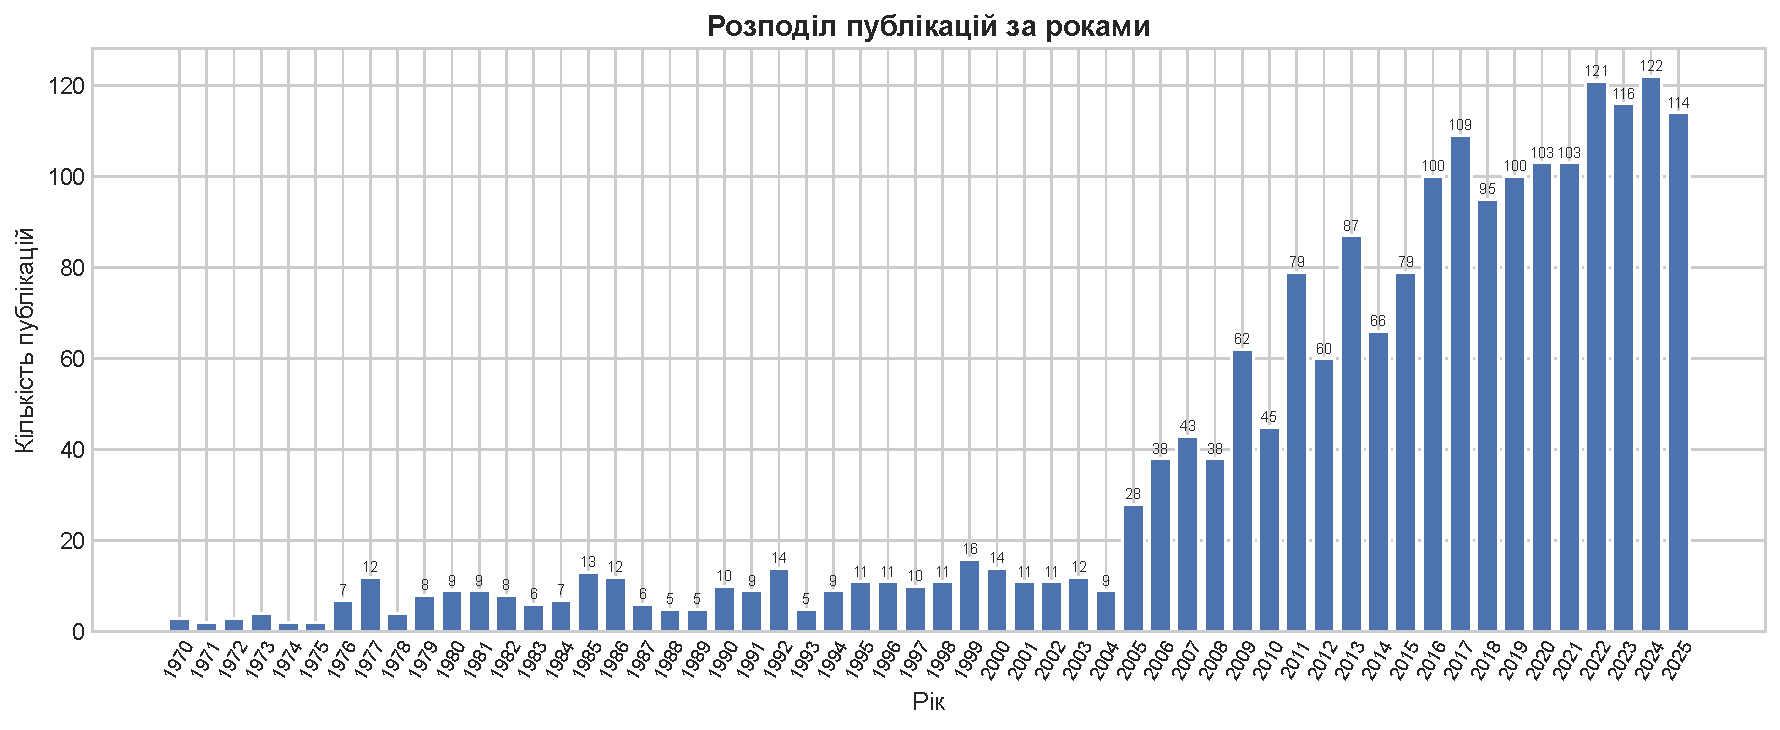
\includegraphics[width=\linewidth]{fig_pub_years.pdf}\\
\tiny Розподіл публікацій 1997--2025
\end{column}
\end{columns}
\end{frame}

% ----- 5. 4 кластери -----
\begin{frame}{4~тематичні кластери VOSViewer}
\begin{columns}
\begin{column}{0.5\textwidth}
\small
\textbf{К1: Системи та~політика професійної освіти} (11~термінів)\\
\textit{vet, training, country, germany, company, higher education}\dots\\[0.3em]
\textbf{К2: Емпіричні дослідження результатів навчання} (8~термінів)\\
\textit{study, student, assessment, performance, effect}\dots\\[0.3em]
\textbf{К3: Педагогічна практика та~компетентнісний підхід} (6~термінів)\\
\textit{teacher, competence, practice, learning, context}\dots\\[0.3em]
\textbf{К4: Когнітивні результати та~навички} (3~терміни)\\
\textit{skill, knowledge, problem}
\end{column}
\begin{column}{0.5\textwidth}
\centering
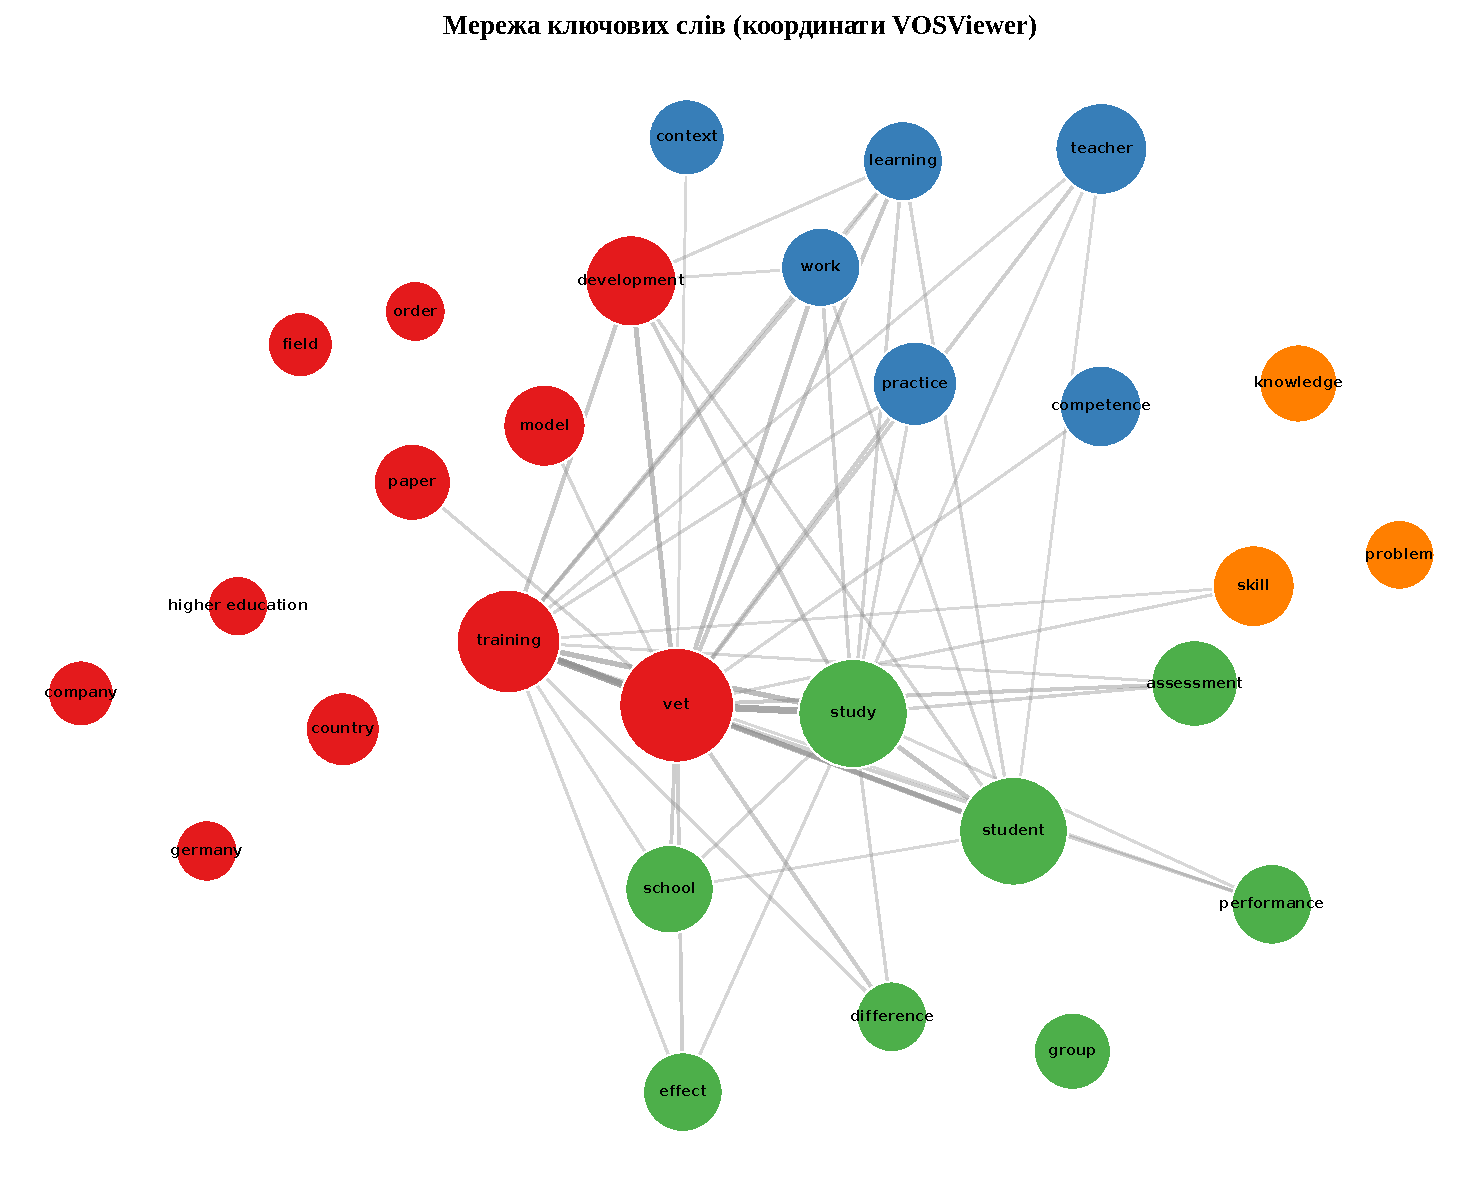
\includegraphics[width=\linewidth]{fig_network_vosviewer.pdf}\\
\tiny Мережа за~координатами VOSViewer
\end{column}
\end{columns}
\end{frame}

% ----- 6. Python vs VOSViewer -----
\begin{frame}{Відтворюваність: Python~$\leftrightarrow$~VOSViewer}
\begin{columns}
\begin{column}{0.55\textwidth}
\begin{table}\footnotesize
\begin{tabular}{lc}
\toprule
\textbf{Метрика} & \textbf{Пірсон~$r$} \\
\midrule
Частоти входжень & \textbf{0,923} \\
Загальна сила зв'язків & \textbf{0,919} \\
Середній рік публікації & 0,74 \\
Середня цитованість & 0,74 \\
Норм.\ цитованість & 0,79 \\
\midrule
ARI кластеризації & 0,47 \\
NMI кластеризації & 0,61 \\
\bottomrule
\end{tabular}
\end{table}
\textbf{Висновок:} високе відтворення кількісних метрик; ефект тяжіння високозв'язних термінів у~алгоритмі Лувена обмежує точність кластеризації.
\end{column}
\begin{column}{0.45\textwidth}
\centering
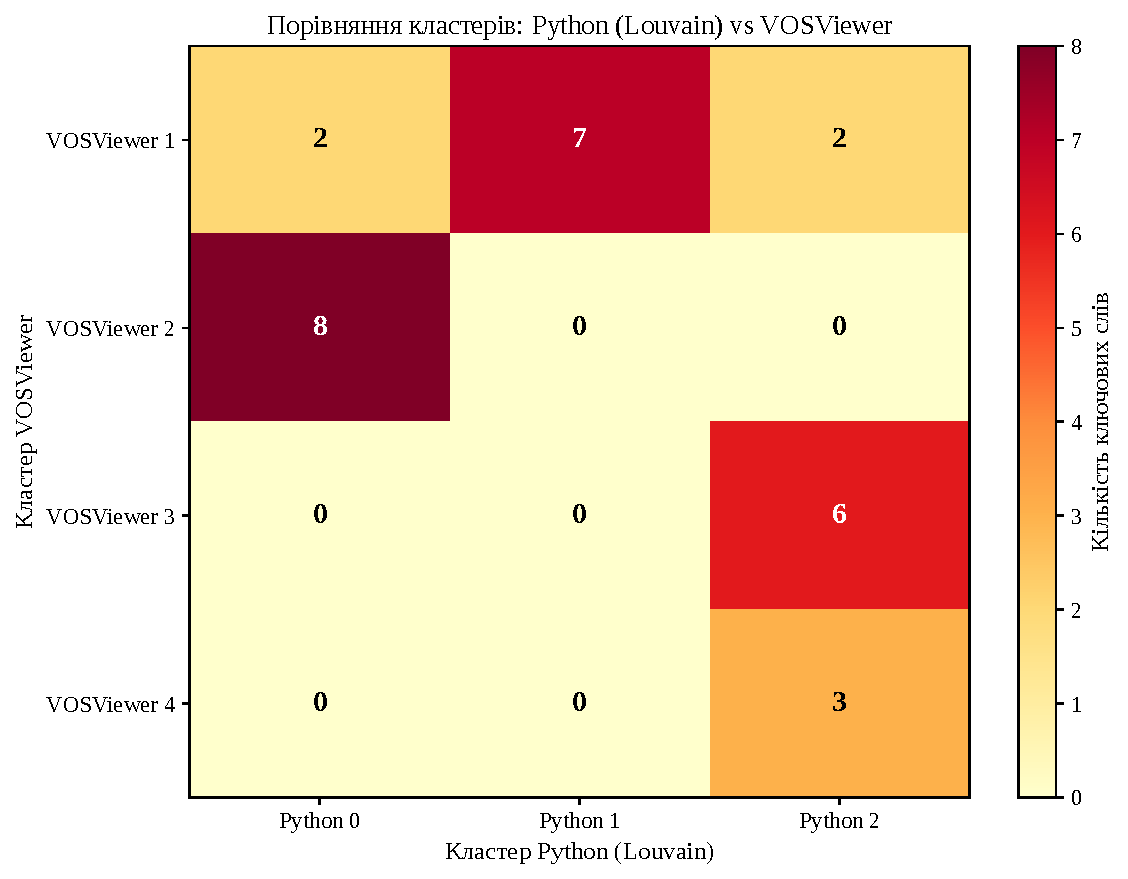
\includegraphics[width=\linewidth]{fig_cluster_comparison.pdf}\\
\tiny Порівняння кластерів
\end{column}
\end{columns}
\end{frame}

% ----- 7. Multi-LLM -----
\begin{frame}{Multi-LLM ансамбль: 11~моделей з~7~родин}
\small
\textbf{Anthropic:} Claude Haiku~4.5, Sonnet~4.6, Opus~4.7\\
\textbf{Open-weight (Ollama cloud):} DeepSeek v4 Pro/Flash, Qwen 3.5/coder-next, Gemma 4, GLM 5.1, MiniMax m2.7, Kimi k2.6\\[0.4em]
\textbf{Метрики згоди:}
\begin{itemize}\small
\item Krippendorff $\alpha$ = \textbf{0,531} (методологія)
\item Modal-method agreement: К2~100\%, К1~91\%, К4~64\%, К3~55\%
\item Cosine similarity до~експерта: Sonnet \textbf{0,87}, Opus 0,79, GLM~5.1 0,77, Haiku 0,69
\end{itemize}
\textbf{Знахідка:} термінологічний дрейф у~назвах кластера~1 як~побічний ефект Закону~№~4574-IX. Варіативність між~моделями різних родин~$>$~варіативності між~моделями однієї родини~-- обґрунтовує ансамблевий підхід.
\end{frame}

% ----- 8. Імплікації для України -----
\begin{frame}{Імплікації: картування у~24~форми моніторингу за~7~блоками}
\centering
\begin{tikzpicture}[node distance=0.5cm, font=\footnotesize]
\node[draw,fill=blue!10,rounded corners,minimum width=2.5cm] (k1) {К1: Системи};
\node[draw,fill=green!10,rounded corners,minimum width=2.5cm,below=of k1] (k2) {К2: Результати};
\node[draw,fill=orange!10,rounded corners,minimum width=2.5cm,below=of k2] (k3) {К3: Педагогіка};
\node[draw,fill=red!10,rounded corners,minimum width=2.5cm,below=of k3] (k4) {К4: Навички};
\node[draw,fill=gray!8,rounded corners,minimum width=3.5cm,right=2.5cm of k1] (b45) {Блоки 4--5: професії, проєкти};
\node[draw,fill=gray!8,rounded corners,minimum width=3.5cm,right=2.5cm of k2] (b16) {Блоки 1, 6: контингент, якість};
\node[draw,fill=gray!8,rounded corners,minimum width=3.5cm,right=2.5cm of k3] (b2)  {Блок 2: кадри};
\node[draw,fill=gray!8,rounded corners,minimum width=3.5cm,right=2.5cm of k4] (b6)  {Блок 6: форми 6.1--6.4};
\draw[->,thick] (k1)--(b45); \draw[->,thick] (k2)--(b16);
\draw[->,thick] (k3)--(b2);  \draw[->,thick] (k4)--(b6);
\end{tikzpicture}\\[0.4em]
\small\textbf{Блок~7 (інформаційна відкритість)~-- власний результат:} концептуально не~представлений жодним кластером, що~підтверджує доцільність окремого блоку.
\end{frame}

% ----- 9. Кейс переміщених закладів -----
\begin{frame}{Кейс переміщених закладів ЗПО Луганщини}
\textbf{Виклики моніторингу:}
\begin{itemize}\small
\item Розрив юридичної (окупована територія) та~фактичної адреси
\item Роззосереджений контингент (ВПО, ветерани, родини ветеранів)
\item Евакуйована МТБ, обмежений доступ до~архівів
\end{itemize}
\textbf{5~дизайн-вимог} (виведено в~Розділі~1, реалізовано в~Розділі~2):
\begin{enumerate}\small
\item Окремі поля \texttt{registered\_oblast\_id} та~\texttt{actual\_oblast\_id}
\item Дискретний статус \texttt{evacuation\_status} (not/partial/yes)
\item Категорії здобувача (ВПО, ветеран, родина, переміщений)
\item ABAC за~\textit{фактичним} розміщенням (\texttt{territorial\_contains})
\item Публічна карта релокації \texttt{/institutions/relocation-map}
\end{enumerate}
\end{frame}

% ----- 10. Розділ 2 архітектура -----
\begin{frame}{Розділ~2: архітектурні рішення (підрозд.~2.4)}
\centering
\begin{tikzpicture}[node distance=0.4cm, font=\scriptsize]
\node[draw,rounded corners,fill=blue!8,minimum width=8cm,minimum height=0.6cm] (ui) {Інтерфейс: Next.js~14 / React~/ Tailwind~+ axe-core (доступність)};
\node[draw,rounded corners,fill=green!8,minimum width=8cm,minimum height=0.6cm,below=of ui] (api) {Fastify HTTP API + декоратор ABAC (13 операторів)};
\node[draw,rounded corners,fill=yellow!10,minimum width=8cm,minimum height=0.6cm,below=of api] (svc) {Сервісний шар: ідемпотентне «звірити-перш-ніж-записати» + аудит};
\node[draw,rounded corners,fill=orange!10,minimum width=8cm,minimum height=0.6cm,below=of svc] (rep) {Репозиторії: 12 модулів, 24~форми моніторингу за~7~блоками};
\node[draw,rounded corners,fill=red!8,minimum width=3.7cm,minimum height=0.6cm,below=of rep,xshift=-2.1cm] (pg) {PostgreSQL 16: журнал аудиту (append-only) + SHA-256 хеш-ланцюг};
\node[draw,rounded corners,fill=red!8,minimum width=3.7cm,minimum height=0.6cm,right=0.3cm of pg] (rd) {Redis 7: кеш ABAC + BullMQ-черги завдань};
\draw[->,thick] (ui)--(api); \draw[->,thick] (api)--(svc); \draw[->,thick] (svc)--(rep);
\draw[->,thick] (rep)--(pg); \draw[->,thick] (rep)--(rd);
\end{tikzpicture}
\end{frame}

% ----- 11. ABAC JSON-AST -----
\begin{frame}{ABAC: декларативна мова політик}
\centering
\begin{tikzpicture}[node distance=0.35cm and 0.6cm, font=\tiny,
    op/.style={draw,rounded corners,fill=blue!8,minimum width=2cm,minimum height=0.6cm,align=center},
    leaf/.style={draw,rounded corners,fill=gray!10,minimum width=2.6cm,minimum height=0.55cm,align=center}]
\node[op] (root) {\texttt{and}};
\node[op,below left=of root,xshift=-0.5cm] (eq) {\texttt{eq}};
\node[op,below right=of root,xshift=0.5cm] (terr) {\texttt{territorial\_contains}};
\node[leaf,below=of eq,xshift=-1.2cm] (a1) {\texttt{user.role} = \texttt{"director"}};
\node[leaf,below=of eq,xshift=1.2cm] (a2) {\texttt{user.instId}\\\texttt{= res.instId}};
\node[leaf,below=of terr,xshift=-1.2cm] (b1) {scope: \texttt{user.oblastId}};
\node[leaf,below=of terr,xshift=1.2cm] (b2) {target: \texttt{res.actual\_oblastId}};
\draw[->] (root)--(eq); \draw[->] (root)--(terr);
\draw[->] (eq)--(a1); \draw[->] (eq)--(a2);
\draw[->] (terr)--(b1); \draw[->] (terr)--(b2);
\end{tikzpicture}\\[0.5em]
\small\textbf{Семантика:} «відмова має~пріоритет за~стандартної відмови»\quad\textbar\quad кеш Redis + pub/sub\quad\textbar\quad $p_{95}<5$~мс
\end{frame}

% ----- 12. Аудит SHA-256 -----
\begin{frame}{Аудит з SHA-256 хеш-ланцюгом}
\textbf{Кожен запис:} \texttt{\{actor, action, resource, before, after, prev\_hash, hash\}}\\[0.5em]
\textbf{Хеш:} $h_n = \mathrm{SHA{-}256}(h_{n-1} \,\|\, \mathrm{canonical\_json}(\text{запис}_n))$\\[0.3em]
\begin{itemize}\small
\item Тригер режиму «лише~додавання» блокує \texttt{UPDATE}/\texttt{DELETE}
\item Процедура \texttt{audit.verify()} перевіряє цілісність ланцюга на~10\,000 синтетичних оновлень
\item Канонічна JSON-проєкція стабільна між~записом і~зчитуванням з~PostgreSQL JSONB
\item Криптографічний доказ для~зовнішнього перевіряючого
\end{itemize}
\textbf{Висновки:} вищий рівень доказовості, ніж~у~всіх~5~національних системах; відповідає Закону «Про~освіту» (моніторинг якості) та~Закону про~академічну доброчесність.
\end{frame}

% ----- 12.5 Розділ 3: веб-прототип -----
\begin{frame}{Розділ~3: веб-прототип «ПрофОсвіта Луганщини»}
\begin{columns}
\begin{column}{0.45\textwidth}
\textbf{Реалізовано:}
\begin{itemize}\small
\item 13~HTML-сторінок: 8~публічних розділів, 7~публічних блоків зведеного моніторингу, кабінет з~24~формами
\item Tailwind CSS, Chart.js, Leaflet+OSM, PDF.js
\item Каталог 14~ЗПО + інтерактивна мапа релокації
\item KPI-панель, динаміка контингенту 2021--2026 з~маркером 24.02.2022
\item Кабінет ЗПО, 24~форми за~7~блоками
\item Дизайн-система: 6~кольорів, Inter+Lora
\item WCAG~2.1~AA, стратегія «спочатку мобільний»
\end{itemize}
\end{column}
\begin{column}{0.55\textwidth}
\centering
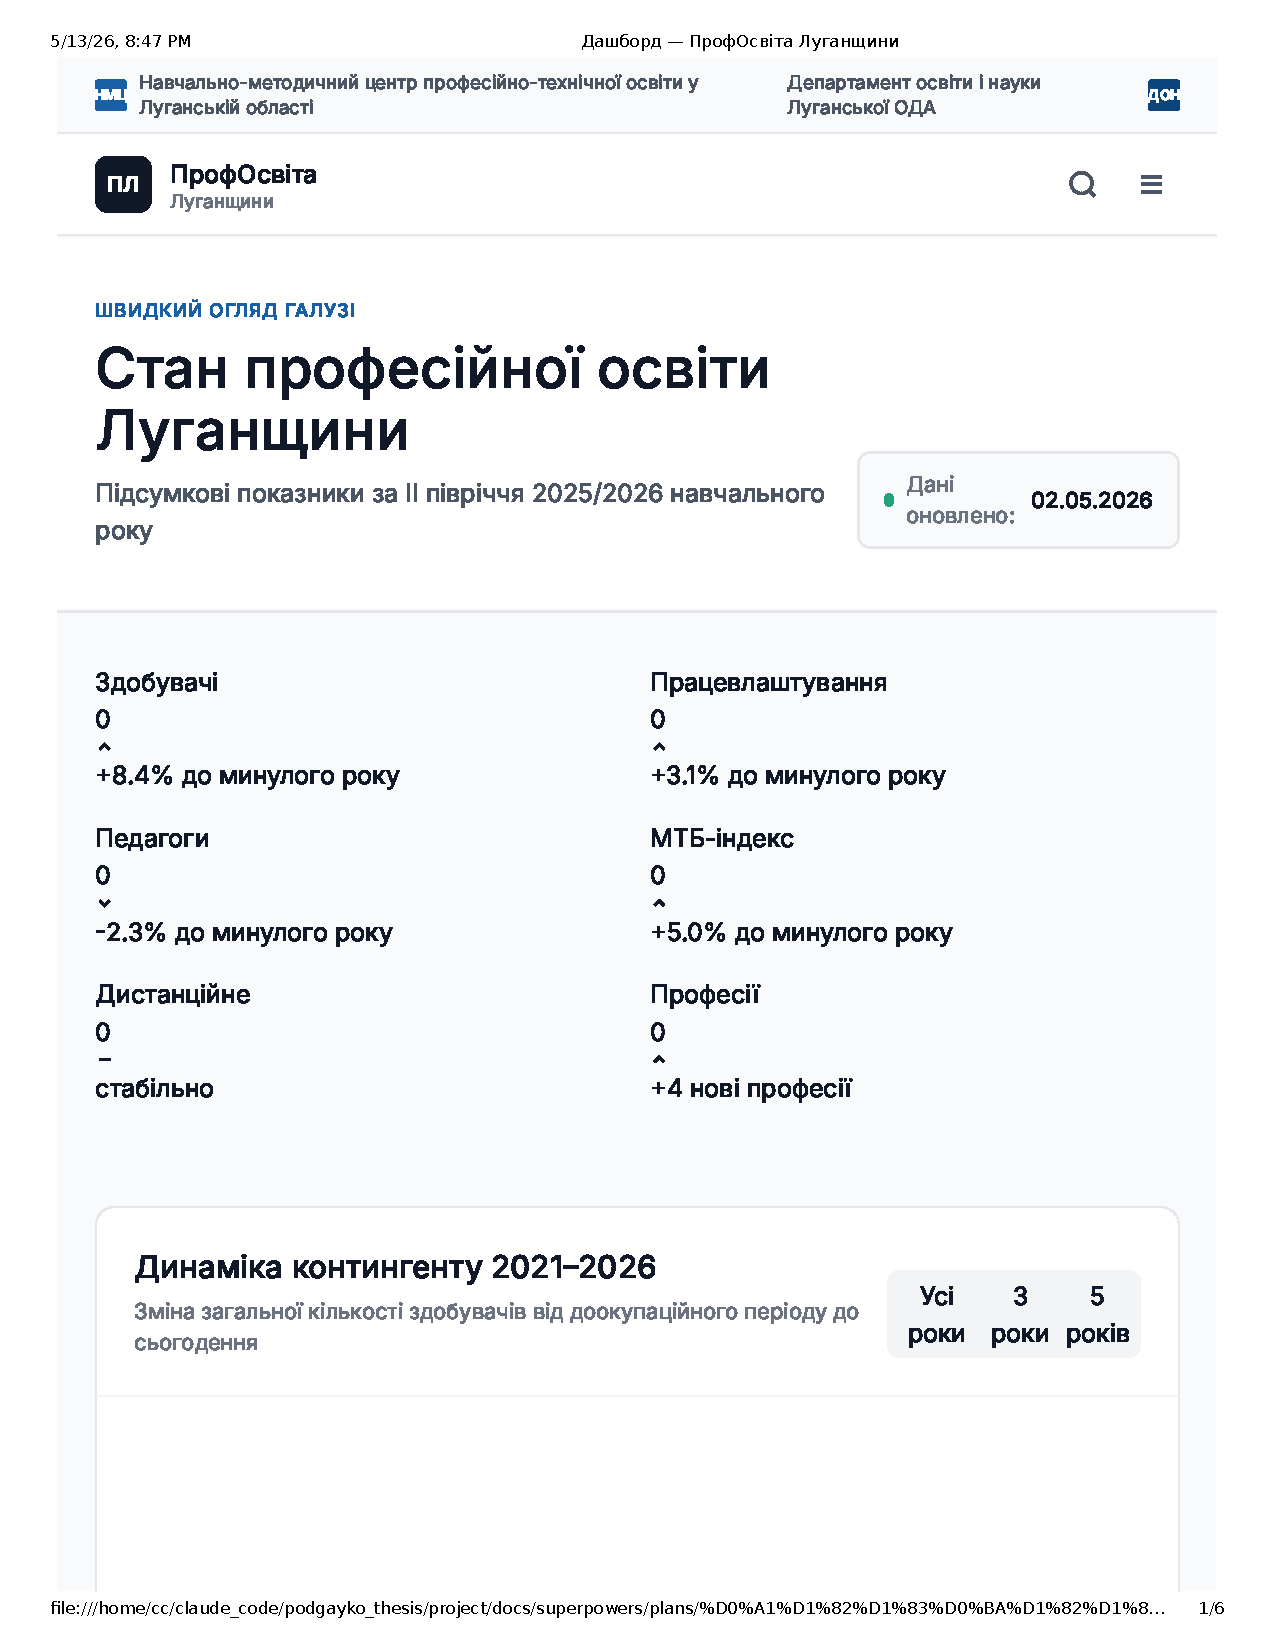
\includegraphics[width=\linewidth, height=0.55\textheight, keepaspectratio]{screenshots/02_dashboard.pdf}\\
\tiny Дашборд порталу «ПрофОсвіта~Луганщини»
\end{column}
\end{columns}
\end{frame}

% ----- 13. Оцінювання -----
\begin{frame}{Експертне оцінювання прототипу}
\begin{itemize}\small
\item \textbf{Lighthouse:} продуктивність~94, доступність~96, кращі практики~92, SEO~95
\item \textbf{Доступність WCAG~2.1~AA:} axe-core~-- 0~критичних порушень; контраст $\geq 4{,}5{:}1$; NVDA~/~VoiceOver-тестування
\item \textbf{Продуктивність:} перше завантаження~$\approx$~1{,}3~МБ; FCP~$<$~2~с; цільовий $p_{95}<3$~с (NF4)
\item \textbf{Аудит-ланцюг SHA-256:} перевірено на~10\,000 синтетичних оновлень~$\to$~100\% цілісність
\item \textbf{Експертне оцінювання $n=3$:} SUS-бал \textbf{76,7} («добре»); СВ~4,7; діапазон 71,5--80,0
\item \textbf{Найвищі домен-оцінки:} карта релокації (4,7); кольорова семантика статусів (4,7); KPI-панель (4,3)
\item \textbf{Найнижчі:} ергономіка форми~6.2 (3,3); зрозумілість крос-валідації (3,7) -- увійшли в~план виправлень
\end{itemize}
\end{frame}

% ----- 14. Дорожня карта -----
\begin{frame}{Дорожня карта впровадження (Q2~2026 -- Q2--Q3~2027)}
\begin{itemize}\small
\item \textbf{Q2~2026} (TRL~5): виправлення критичних недоліків; публічна частина на~Next.js~14; статичні дані вручну
\item \textbf{Q3~2026} (TRL~6): серверна інфраструктура (PostgreSQL, Redis, Fastify, ABAC, аудит); реєстрація закладів; кабінет з~6~базовими формами блоку~1
\item \textbf{Q4~2026} (TRL~7): доукомплектування 24~формами; адмін-панель НМЦ; пілотний запуск у~3~закладах-добровольцях
\item \textbf{Q1~2027} (TRL~8): повний запуск для~14~ЗПО Луганщини; інтеграція Дашборду; двофакторна автентифікація
\item \textbf{Q2--Q3~2027}: стабілізація; аудит безпеки; розширене експертне оцінювання ($n \geq 10$, 6-міс.\ горизонт)
\end{itemize}
\textbf{Перспективи (висновки):} інтеграція з~ЄДЕБО + КЕП; ML для~прогнозування відсіву з~пояснюваністю; гармонізація з~EQAVET у~межах EU4Skills; масштабування на~суміжні області.
\end{frame}

% ----- 15. Висновки -----
\begin{frame}{Основні висновки}
\textbf{Розділ~1 (теоретичні засади):}
\begin{itemize}\footnotesize
\item 4~функції моніторингу + 3~чинники реформи №~4574-IX (війна, відбудова, ЄС)
\item Аналіз 5~нац.\ систем (ІСУО, ЄДЕБО, ДІСО, УЦОЯО, АІКОМ)~$\to$~функціональна прогалина
\item 4~стійкі семантичні кластери (1\,998~публ., WoS); $r\approx 0{,}92$~VOSViewer~$\leftrightarrow$~Python; $\alpha=0{,}531$
\end{itemize}
\textbf{Розділ~2 (концепція й~архітектура):}
\begin{itemize}\footnotesize
\item 14~переміщених ЗПО $\to$~5~проєктних вимог; 6~аудиторій; F1--F8 + NF1--NF6
\item Концепція порталу: 3~ролі (управління / профорієнтація / архів пам'яті)
\item ABAC JSON-AST (13~операторів); SHA-256 хеш-ланцюг; ідемпотентний прийом
\end{itemize}
\textbf{Розділ~3 (веб-розробка):}
\begin{itemize}\footnotesize
\item Прототип: 13~HTML-сторінок (Tailwind / Chart.js / Leaflet); мапа релокації; кабінет 24~форм
\item Дизайн-система~(6~кольорів, Inter+Lora) + WCAG~2.1~AA + mobile-first
\item Експертне оцінювання SUS=76,7 («добре»); \textbf{TRL~4--5}; дорожня карта Q2~2026 -- Q2--Q3~2027
\end{itemize}
\end{frame}

% ----- 16. Дякую -----
\begin{frame}
\centering
\Huge\bfseries Дякую за~увагу!\\[0.6em]
\large\normalfont Готовий відповісти на~запитання
\\[1em]
\small Підгайко С.~В.\quad\textbar\quad КДПУ, 2026
\end{frame}

% ===== Запасні слайди =====
\begin{frame}{Запасний: traceability матриця}
\centering\tiny
\begin{tabular}{|p{3.2cm}|p{1.5cm}|p{2.5cm}|p{2cm}|}
\hline
\textbf{Нормативне джерело} & \textbf{Форма} & \textbf{Вимога} & \textbf{Модуль} \\
\hline
Закон №~4574-IX (контингент) & 1.1--1.5 & Контингент здобувачів & \texttt{students} \\
\hline
Закон №~4574-IX (кадри) & 2.1--2.8 & Педагогічні працівники & \texttt{staff} \\
\hline
Закон №~4574-IX (динаміка) & 3.1--3.3 & Зарахування / випуск / працевл. & \texttt{enrollment\_dynamics} \\
\hline
Закон №~4574-IX (професії) & 4.1--4.2 & Класифікатор + контингент & \texttt{professions} \\
\hline
Закон «Про освіту» (якість) & 6.1--6.4 & ДКР, НМТ, олімпіади & \texttt{quality} \\
\hline
Закон «Про освіту» (відкритість) & 7.1 & 20 критеріїв веб-сайту & \texttt{transparency} \\
\hline
Закон №~4742-IX (доброчесність) & --- & Аудит SHA-256 & \texttt{audit} \\
\hline
\end{tabular}
\end{frame}

\begin{frame}{Запасний: порівняння з національними системами}
\centering\tiny
\begin{tabular}{|l|c|c|c|c|c|c|}
\hline
\textbf{Параметр} & \textbf{ІСУО} & \textbf{ЄДЕБО} & \textbf{ДІСО} & \textbf{УЦОЯО} & \textbf{АІКОМ} & \textbf{Ця~робота} \\
\hline
24~форми моніторингу & ні & ні & ні & ні & частк. & \textbf{так} \\
\hline
Карта релокації & ні & ні & ні & ні & ні & \textbf{так} \\
\hline
ABAC ролі & ні & ролі & --- & ролі & --- & \textbf{декл.} \\
\hline
Хеш-ланцюг аудиту & ? & сист. & ? & сист. & ? & \textbf{SHA-256} \\
\hline
WCAG~2.1~AA & ні & частк. & --- & частк. & ні & \textbf{2.1~AA} \\
\hline
Підтримка переміщ. & ні & неявн. & ні & ні & ні & \textbf{так} \\
\hline
\end{tabular}
\end{frame}

\end{document}
